\documentclass[11pt]{article}
\usepackage[T1]{fontenc}
\usepackage[utf8]{inputenc}
\usepackage{lmodern}
\usepackage{royden-report}
\usepackage{microtype,longtable,array,enumitem}
\setlist{topsep=5pt,itemsep=3pt,parsep=0pt}
\setlength{\emergencystretch}{2em}
\widowpenalty=10000
\clubpenalty=10000
\newcolumntype{P}[1]{>{\raggedright\arraybackslash}p{#1}}
\newcommand{\ii}{\mathrm{i}}
\newcommand{\dd}{\,\mathrm{d}}
\newcommand{\norm}[1]{\left\lVert#1\right\rVert}
\newcommand{\abs}[1]{\left\lvert#1\right\rvert}
\DeclareMathOperator{\Impart}{Im}
\DeclareMathOperator{\Repart}{Re}
\DeclareMathOperator{\Arg}{Arg}
\hypersetup{pdftitle={Nonlinear Schrodinger equations and physics-informed learning},pdfauthor={Research review prepared for the Dysthe project}}
\title{Nonlinear Schr\"odinger Equations\\and Physics-Informed Learning}
\author{Research review and a water-wave Dysthe agenda}
\date{Literature cutoff: 25 October 2026}
\begin{document}
\maketitle
\begin{abstract}
Physics-informed neural networks have been used to approximate nonlinear
Schr\"odinger solutions, infer coefficients, reconstruct fields from sparse
observations, and learn reusable solution operators. These are different
tasks, and progress on one does not establish superiority on the others.
This review separates direct NLS evidence, water-wave evidence, transferable
training methods, and very recent work with limited accessible evidence.
The recommended first project asks whether the approved spatial Dysthe
equation improves sparse-observation reconstruction and downstream prediction
beyond retuned NLS and classical numerical assimilation. Five concrete
research questions, a reproducible benchmark, and a staged plan are provided.
No published experiment was independently reproduced for this review.
\end{abstract}
\tableofcontents
\section{Recommendation and review method}
\label{sec:recommendation}
\paragraph{Recommended first paper.}
Ask: \emph{When does spatial Dysthe physics improve reconstruction and
downstream prediction from sparse water-wave observations, after NLS is
allowed to fit effective coefficients?} The contribution should be a
validated map of when the additional physics is useful, including
uncertainty and computational cost. It should not rest solely
on substituting a more complicated residual into a familiar neural network.

The clearest published motivation is Ehlers et al.'s water-wave NLS study,
whose Conclusions propose Dysthe as a next model \cite{ehlers2024}.
However, subsequent papers already address fully nonlinear wave
reconstruction and reusable physics-informed operators
\cite{ehlers2025,wavepino}. Therefore, generic claims of the first PINN
for water-wave reconstruction or a fast water-wave PINO are unsuitable.
The more defensible opportunity is a controlled comparison of physics,
identifiability, phase accuracy, and generalization in the specified equation.

\paragraph{What newest and best mean here.}
This is a targeted critical review of primary literature available by
25 October 2026, not an exhaustive systematic review or a universal ranking.
Searches combined NLS/Schr\"odinger, PINN, water waves, Dysthe,
conservation, causal training, optimization, error bounds, sparse
assimilation, and operator learning; recent searches emphasized 2024--2026.
Publisher records, author manuscripts, proceedings, author code, and data
repositories were consulted. Publication status was checked separately from
arXiv submission dates. The source ledgers supplied with the report record
access and limitations. A search failure is not proof of absence.

Priority is based on relevance to the task, quality of comparisons,
independent test data, access to methods and code, and clarity about costs.
There is no common benchmark establishing one best NLS--PINN method across
forward, inverse, long-distance, and many-query problems. Numerical errors
reported on different domains, norms, equations, and data budgets are not a
leaderboard. Very recent publisher abstracts are useful leads, but provide
less inspectable evidence than a complete manuscript and executable release.

\paragraph{Reading priorities.}
Read Ehlers et al. (2024) for the direct research motivation;
Urb\'an et al. (2025) for a serious compact NLS training baseline;
Zhang et al. (2025) for complex-valued NLS learning;
Hao et al. (2026) for hard-constraint ablations;
and the 2025 water-wave PINO paper for the many-query comparison
\cite{ehlers2024,urban,cvpinn,hardic,wavepino}.
Read the 2026 GRAVIS, Noether, and phase--amplitude papers as recent
method candidates, with the access limitations in Section~\ref{sec:literature}.
For a mathematics-led direction, add Alejo et al. and Eiras et al.
\cite{alejo,eiras}.

\paragraph{Evidence labels.}
Throughout this report, \emph{reported} means an author's result, not a result
reproduced here. \emph{Explicit future work} identifies an actual statement
in the inspected source. \emph{Proposed question} is this review's synthesis.
An available code repository is evidence of availability, not evidence that
the code reproduces every claim. The figures in this report are original
analytic illustrations and experiment diagrams, not new PINN experiments.

\paragraph{Scope.}
The literature survey concerns NLS methods broadly. All proposed active
research stays within unidirectional deep-water gravity waves and the
one-profile-coordinate spatial free-surface model
\texttt{water-wave-dysthe-spatial-v1}. General NLS, higher-order NLS, and
other Schr\"odinger demonstrations can motivate algorithms; they are not
water-wave Dysthe validation. Changes of formulation, dimension, or
coefficients require explicit separate model identities.

\section{The PDE and the learning tasks}
\label{sec:math}
\subsection{What NLS describes}
An envelope describes the slowly varying amplitude and phase of an
oscillatory wave. For example, a leading-order surface signal has the form
\[
 \eta(x,t)\approx\Repart\{B(x,t)e^{\ii(k_0x-\omega_0t)}\}.
\]
The complex field $B$ contains information about both the height and the
position of the carrier oscillations. Matching $|B|$ alone therefore does
not ensure accurate surface-wave prediction. Envelope-to-surface conversion,
including any retained bound harmonics, must be specified consistently.

A common mathematical normalization of cubic NLS is
\begin{equation}
 \ii q_s+p q_{yy}+\gamma |q|^2q=0,
 \qquad (s,y)\in[0,S]\times\mathbb T_L,
 \label{eq:nls}
\end{equation}
where $q$ is complex, $s$ is an evolution variable, $y$ is a profile
coordinate, $p,\gamma\in\RR$, and $\mathbb T_L=\RR/(L\mathbb Z)$.
Dispersion is represented by $p q_{yy}$ and nonlinear phase modulation by
$\gamma|q|^2q$. Under this convention $p\gamma>0$ is the focusing case;
$p\gamma<0$ is the defocusing case. Signs and scalings vary across papers.
An equation written in laboratory time is not automatically the same
experimental problem as spatial propagation of a retarded-time envelope.

Bright solitons, dark solitons on a background, breathers, and rogue-wave
profiles supply useful test cases. They should not substitute for testing
general random packets, interactions, changed initial conditions, or noisy
observations. Higher-order, variable-coefficient, coupled, and nonlocal NLS
models introduce further terms and may have different invariants and
well-posedness assumptions.

For smooth periodic solutions of \eqref{eq:nls}, standard conserved
quantities are mass (or action), momentum, and Hamiltonian:
\begin{align}
 M[q]&=\int_{\mathbb T_L}|q|^2\dd y,&
 P[q]&=\Impart\int_{\mathbb T_L}\overline q q_y\dd y,\notag\\
 H[q]&=\int_{\mathbb T_L}
       \left(p|q_y|^2-\frac{\gamma}{2}|q|^4\right)\dd y.
 \label{eq:nlsinvariants}
\end{align}
These expressions assume the stated normalization and boundary conditions.
On the real line, their use also requires suitable integrability. They are
not a license to impose the same constraints on a different envelope model.

\subsection{How a PINN is used}
A conventional PINN represents $q_\theta=a_\theta+\ii b_\theta$ by two real
network outputs. Its NLS residual has real and imaginary parts
\begin{align*}
 r_a&=-\partial_s b_\theta+p\partial_{yy}a_\theta
          +\gamma(a_\theta^2+b_\theta^2)a_\theta,\\
 r_b&=\partial_s a_\theta+p\partial_{yy}b_\theta
          +\gamma(a_\theta^2+b_\theta^2)b_\theta.
\end{align*}
Automatic differentiation supplies the local derivatives. Complex-valued
networks instead use complex internal parameters or operations; both
representations can express a complex solution. Their relative usefulness
is an empirical question about trainability and inductive bias.

A representative objective is
\begin{equation}
 \mathcal L=\lambda_r\sum_j w_j|r_\theta(z_j)|^2
  +\lambda_0\mathcal L_0+\lambda_b\mathcal L_b
  +\lambda_d\mathcal L_d+\lambda_I\mathcal L_I.
 \label{eq:loss}
\end{equation}
Here $z_j=(s_j,y_j)$ are residual points; $\mathcal L_0$ and
$\mathcal L_b$ measure initial and boundary errors;
$\mathcal L_d$ compares an observation operator applied to $q_\theta$
with data; and $\mathcal L_I$ optionally measures invariant defects.
Weights require scaling and validation. A small value of this sampled,
weighted objective is not itself a bound on the solution error. This basic
framework has a direct NLS precedent in Raissi et al. \cite{raissi}.

\begin{longtable}{@{}P{0.17\textwidth}P{0.35\textwidth}P{0.40\textwidth}@{}}
\toprule
Task & What is learned & Appropriate test \\
\midrule
Forward solve & A field for one specified initial condition and PDE. &
Error and total solve time against a converged numerical solution. \\
Inverse problem & Coefficients, latent initial field, or both, from observations. &
Identifiability, noisy-data robustness, and withheld observations. \\
Assimilation & A consistent field over the observed region. &
Reconstruction at withheld locations; distinguish interpolation from forecast. \\
Operator learning & A map from initial fields or measurements to solution fields. &
Completely unseen trajectories and amortized cost including training. \\
\bottomrule
\end{longtable}
A network trained on one soliton does not become a general solution operator
because it can be evaluated at arbitrary coordinates. A PINO or
physics-informed DeepONet is trained across inputs to learn such a map
\cite{pino}. The same distinction applies to sensor-conditioned models.

\subsection{The approved water-wave Dysthe equation}
The current project contract specifies
\begin{equation}
\begin{split}
 u_\xi={}&-\ii u_{\tau\tau}-\ii|u|^2u\\
 &-\varepsilon\left(8|u|^2u_\tau
       +2u^2\overline{u_\tau}
       +2\ii u\,|D_\tau|(|u|^2)\right).
\end{split}
\label{eq:dysthe}
\end{equation}
Here $\xi$ is propagation distance, $\tau$ is retarded time, $u$ is the
scaled free-surface envelope, and $\varepsilon$ is carrier steepness in the
specified formal normalization. This convention agrees with the
free-surface equation (1.3) of Fedele--Dutykh \cite{fedele}. In the source
coordinates, $\tau=\varepsilon(2x-t)$, $\xi=\varepsilon^2x$, and
$B=\varepsilon u$. Setting $\varepsilon=0$ defines a mathematical NLS
control; the physical coordinate map is not invertible at zero steepness.

On periodic profiles, the nonlocal operator is
\[
 \widehat{|D_\tau|f}(k)=|k|\widehat f(k),
 \qquad k=2\pi n/L,\quad n\in\mathbb Z.
\]
For the forward Fourier convention $e^{-\ii k\tau}$,
$|D_\tau|=\mathcal H\partial_\tau$; its zero mode is zero. This term
depends on the full profile. Differentiating a pointwise neural output at
isolated random points does not evaluate this operator.

The free-surface field is noncanonical. Use the correct transformed
invariants and boundary convention if imposing an energy or momentum
constraint. The potential-envelope equation, whose corresponding
conjugate-derivative coefficient is zero, is a different formulation.
The shared model file also requires periodic grids without a duplicated
endpoint, complex arrays with axes $(\xi,\tau)$, and whole-initial-field
data splits. Two array axes are not two horizontal physical directions.

\section{Why a good-looking NLS solution is insufficient}
\label{sec:failure}
There are several independent sources of failure: an inappropriate PDE;
insufficient observation information; an unresolved reference calculation;
a network that does not represent the relevant oscillations; and training
that does not reach the relevant solution. Improving an optimizer only
addresses part of this chain.

For oscillatory problems, important practical issues are spectral bias,
imbalanced initial/boundary/residual gradients, large residual regions
dominating small localized events, accumulated phase error, and inconsistent
boundary conditions. Hard constraints, causal weighting, adaptive sampling,
and better curvature information address different mechanisms
\cite{hardic,causal,gravis,urban,soap}.

\begin{example}[Conservation can miss accumulated phase error]
On any periodic profile domain, consider
\[
 q(s,y)=e^{2\ii s},\qquad
 v(s,y)=e^{\ii(2+\delta)s},\qquad \delta\in\RR.
\]
The first solves \eqref{eq:nls} with $p=1$, $\gamma=2$. Both fields have
the same initial data, amplitude, mass, momentum, and Hamiltonian. Yet
\[
 r[v]=-\delta v,\qquad
 \frac{\norm{v(s)-q(s)}_{L^2}}{\norm{q(s)}_{L^2}}
       =2\abs{\sin(\delta s/2)}.
\]
Thus a small persistent residual can accumulate a large phase error.
This is an exact analytic illustration, not a trained-network result.
\end{example}

\begin{figure}[htbp]
\centering
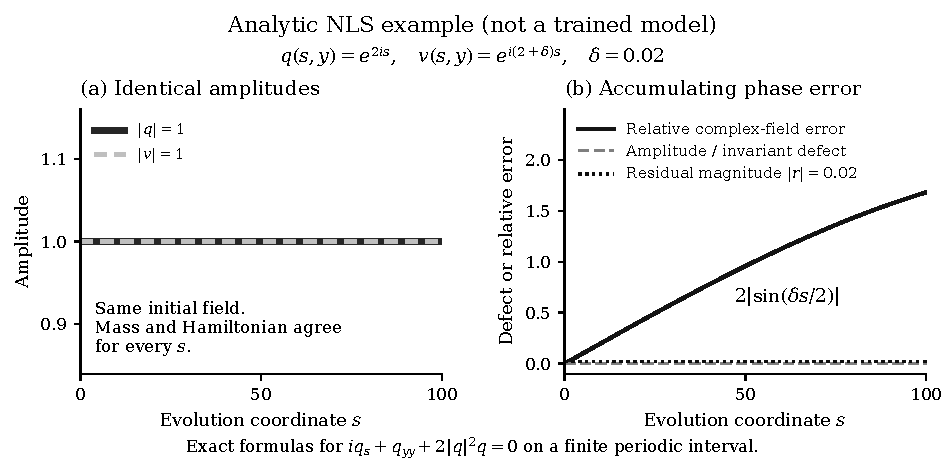
\includegraphics[width=0.95\textwidth]{figures/phase-drift.pdf}
\caption{Exact illustration with $\delta=0.02$. Amplitude and invariant
defects are zero, while complex-field error grows over the plotted interval.
The residual magnitude stays at $0.02$. No PINN or Dysthe experiment is
represented.}
\label{fig:phase}
\end{figure}

\begin{proposition}[A conditional NLS residual estimate]
Let $q,v$ be sufficiently smooth periodic fields on
$[0,S]\times\mathbb T_L$, with $q$ solving \eqref{eq:nls} and
$r=\ii v_s+p v_{yy}+\gamma|v|^2v$. Assume $p,\gamma$ are real and
$|q|,|v|\leq B$ everywhere. Then, for $0\leq s\leq S$,
\begin{equation}
 \norm{v(s)-q(s)}_2\leq e^{3|\gamma|B^2s}
 \left(\norm{v(0)-q(0)}_2+
          \int_0^s\norm{r(t)}_2\dd t\right).
 \label{eq:stability}
\end{equation}
\end{proposition}
\begin{proof}
Set $e=v-q$. The periodic linear Schr\"odinger part contributes zero
to the real $L^2$ energy derivative. The pointwise inequality
$\bigl||v|^2v-|q|^2q\bigr|\leq3B^2|v-q|$ and Cauchy--Schwarz give
$\frac{\mathrm d}{\mathrm ds}\norm e_2
\leq3|\gamma|B^2\norm e_2+\norm r_2$ wherever the norm is nonzero.
Regularization of the norm gives the same integral inequality at its
zeros. Gronwall's inequality yields \eqref{eq:stability}.
\end{proof}
This elementary estimate is included for explanation, not as a novel
theorem. It requires a continuous residual norm, initial-error control, and
amplitude bounds; a training mean-squared error does not supply these
automatically. Its exponential factor can be pessimistic. It does not prove
an analogous estimate for Dysthe's derivative and nonlocal nonlinearities.
The more refined NLS theory discussed below uses different norms and
explicit integration assumptions \cite{alejo}.

\section{The strongest and newest relevant literature}
\label{sec:literature}
\subsection{Direct water-wave evidence}
\paragraph{NLS assimilation and inverse calibration: Ehlers et al. (2024).}
This \emph{Fluids} paper studies 630 synthetic higher-order-spectral (HOS)
wave samples, using observations at two gauge positions and evaluating at
intermediate positions. Fitting carrier-related parameters reduces reported
mean surface similarity parameter (SSP) error from $0.204$ to $0.186$.
Broader spectra and steeper waves remain difficult. The experiments use
numerical data, not a laboratory validation. The paper explicitly proposes
Dysthe residuals, gauge-separation studies, and actual measurements
\cite{ehlers2024}. Its importance is the realistic inverse task and explicit
model discrepancy. Better reconstruction with fitted parameters does not,
by itself, prove that those parameters recover the true physics.

\paragraph{Potential-flow PINNs: Ehlers et al. (2025).}
Published in \emph{Physical Review Fluids} on 2 September 2025, this study
uses elevation and velocity-potential networks with potential-flow
constraints. It includes laboratory flume measurements and reports a
laboratory reconstruction SSP of $0.049$. Forecast quality deteriorates
beyond the assimilation interval; inferred laboratory velocity potential
does not have independent measured ground truth. This is substantial
evidence beyond analytic-soliton fitting, but uses different equations from
the approved envelope model. Pretraining, faster training, and operators
appear in the outlook \cite{ehlers2025}.

\paragraph{Water-wave PINO: Ehlers, Stender and Hoffmann (2025).}
Published in \emph{Physics of Fluids} on 7 October 2025, this paper already
learns sparse-observation reconstruction with an FNO-based physics-informed
operator. It uses 634/211/211 training/validation/test HOS samples and
potential-flow constraints; reported test SSP means are $0.1035$ and
$0.1341$ for two observation configurations. A representative $0.014$\,s
inference time excludes training. These are synthetic, long-crested cases,
not proof of operational ocean forecasting \cite{wavepino}.
Author code is public. A 1,056-sample HOS dataset was released on
8 April 2026 \cite{hosdata}. Availability was checked; neither was run here.
This is the main prior-art obstacle to claiming generic sparse water-wave
operator learning as new.

\subsection{Direct NLS methods to reproduce or compare}
\paragraph{Compact networks and optimization: Urb\'an, Stefanou and Pons (2025).}
The \emph{Journal of Computational Physics} paper is a strong direct
cubic-NLS baseline. Its self-scaled Broyden example uses two hidden layers
of 40 units and reports real/imaginary relative errors of approximately
$(5\pm1,8\pm2)\times10^{-6}$. Hard initial conditions and periodic features
are part of the setup. Its domain differs from the original Raissi
benchmark, expanding from $[-5,5]$ to $[-15,15]$; the nonperiodic
$\operatorname{sech}$ tails become smaller. Consequently the cross-paper
gain cannot be credited to optimization alone. The authors explicitly
suggest further work on modified limited-memory BFGS
\cite{urban}. Reproduce the complete setup before selecting a larger network.

\paragraph{Complex-valued learning: Zhang et al. (2025).}
The \emph{Physical Review Research} CV-PINN paper has particularly useful
accessible evidence: a full manuscript and public implementation. Complex
layers and predictive dynamic monitoring are compared with an approximately
parameter-matched real network across 16 one-dimensional
Gross--Pitaevskii/NLS examples, with three repeats. Some training runs take
approximately two GPU hours. Spectral computations supply reference fields;
this does not show superiority to those solvers. Sampling improvement is
not uniform in every case. The conclusion explicitly proposes richer
residual/solution-gradient sampling \cite{cvpinn}. Treat this as an
architecture and training source, not as water-wave validation.

\paragraph{Hard-constraint ablations: Hao et al. (2026).}
The \emph{Foundations of Data Science} article, early online 8 June 2026,
examines the effect of initial conditions and training stability. Its NLS
combination of hard initial/periodic conditions, self-adaptive weighting,
and mini-batching reports real/imaginary relative errors
$1.80\times10^{-4}$ and $2.58\times10^{-4}$. Code is public
\cite{hardic}. The value lies in ablation and analysis, not the invention of
hard trial functions. The findings do not imply that every noisy inverse
problem should enforce measured initial data exactly. Its numbers should
not be ranked against Urb\'an's numbers without matching the experiments.

\paragraph{Time decomposition and interacting structures: Chen, Li and Yuen (2025).}
Two direct NLS papers study interface-trained time decomposition
(TDD-PINNs) and nonlinear-interaction multi-domain networks (NI-MPINNs).
They include breathers, rogue-wave combinations, and inverse coefficients
with synthetic noise \cite{tdd,interaction}. Their publisher previews report
substantial gains over conventional PINNs. Full comparative budgets and
code were not verified, so the gains are not independently auditable here.
These are relevant precedents for domain decomposition, which should not
be presented as a new idea in a Dysthe application. A spatial formulation
needs propagation-distance slabs, with consistent interface fields.

\paragraph{Transfer between NLS cases: Chen et al. (2024).}
Multi-view transfer learning reuses pretrained NLS information between
related initial/boundary conditions \cite{transfer}. This is a useful
repeated-case comparator, with publisher-level evidence inspected.
Fine-tuning a pretrained solver and learning an input-conditioned operator
are different algorithms. A new study must measure both adaptation cost
and performance on complete unseen wave packets.

\subsection{Very recent 2026 candidates}
\begin{longtable}{@{}P{0.22\textwidth}P{0.35\textwidth}P{0.35\textwidth}@{}}
\toprule
Paper/date & Method and reported evidence & Assessment and access limit \\
\midrule
\endfirsthead
\toprule
Paper/date & Method and reported evidence & Assessment and access limit \\
\midrule
\endhead
GRAVIS, 14 June \cite{gravis} &
Residual magnitude plus output-layer loss-gradient information; seven
localized NLS cases, matched architectures/budgets; reports
$1.56$--$2.37$ times lower errors than RAD. &
Strong recent sampling comparator. Publisher abstract/metadata inspected;
full text, code, and complete cost audit unavailable. Parameter gradients
are not the same as spatial solution gradients. \\
\addlinespace
Noether-constrained PINNs, 5 September issue \cite{noether} &
Dynamic conservation penalties plus adaptive residual sampling; reports
small soliton amplitude error and invariant fluctuations. &
Promising conservation comparator. Abstract-level access; phase,
forecast horizon, repetitions, and matched costs unverified. Soft penalties
do not enforce exact conservation. \\
\addlinespace
CPA-PINNs, 15 October issue \cite{cpa} &
Phase--amplitude representation with continuity, mass and energy penalties;
semiclassical two-dimensional examples and inverse tests with noise. &
Newest verified phase--amplitude candidate here. Publisher preview
inspected; full tables/code unavailable. Defocusing examples do not validate
focusing water-wave instability. \\
\bottomrule
\end{longtable}

These papers justify updating an experimental comparison. They do not
justify calling one method the established best. A separate late watchlist
item is Hu et al.'s \emph{Geometry-Agnostic Data-Driven Discovery of Extreme
Scenarios}, submitted 20 October 2026 \cite{extreme2026}. Its stationary
NLS/coherent-structure examples and proposed extreme-event applications
are not a demonstrated Dysthe forecasting method.

Two WKB-PINN titles were screened but excluded from the confirmed-cutoff
shortlist: DOI \texttt{10.1016/j.cnsns.2026.110653} has a November 2026
issue date without a verified pre-cutoff online date; the exact eligible
date of DOI \texttt{10.1016/j.physd.2026.135394} was not established.
The source ledger retains these uncertainties rather than assigning dates.

\subsection{Transferable methods: useful, with explicit boundaries}
\paragraph{Causality and depth.}
Wang, Sankaran and Perdikaris' causal PINNs weight later evolution stages
according to earlier residuals \cite{causal}. This is not identical to
training separate time windows. PirateNets initializes adaptive residual
gates so that an effectively shallow model gains depth, and combines this
with Fourier embeddings and physics-informed initialization
\cite{pirate}. Neither flagship paper supplied a direct NLS benchmark in
the inspected material. Their application to \eqref{eq:dysthe} is a
testable transfer proposal. PirateNets explicitly points toward
PDE-specific embeddings and operator-learning initialization.

\paragraph{Optimization beyond Adam and L-BFGS.}
The NeurIPS 2025 gradient-alignment paper studies SOAP preconditioning on
ten PDE benchmarks, reporting roughly $2$--$10$ times better accuracy
alongside approximately twice the training expense \cite{soap}.
The inspected text does not establish NLS superiority. Kiyani et al.
provide broader comparisons of self-scaled quasi-Newton methods
\cite{optimizer}. Include a compact quasi-Newton baseline before declaring
that a sophisticated architecture is necessary. Compare wall time to a
target accuracy, not equal optimizer iteration counts.

\paragraph{Operator learning and benchmark discipline.}
Li et al.'s PINO combines data and PDE constraints to learn across input
functions \cite{pino}. That supports the many-query formulation; it is not
evidence for the present Dysthe implementation. PINNacle supplies broader
evidence that method strengths depend on the PDE and problem regime
\cite{pinnacle}. A shared benchmark is more informative than comparing the
best numbers from unrelated papers.

\paragraph{Spectral and goal-oriented residuals are already prior art.}
Spectral informed neural networks replace differential evaluations with
spectral operations \cite{spectral}. Govoeyi and Richter's April 2026
preprint uses dual-weighted-residual ideas for functional-oriented sampling
on Laplace problems \cite{goal}. An operator-budget study explicitly
charges adaptive-sampler residual evaluations \cite{operatorbudget}.
These are relevant precedents; none establishes a solution to the specific
Dysthe nonlocal error-control problem proposed below. Their existence
rules out claiming generic spectral PINNs or generic goal-oriented
sampling as new.

\subsection{Theory and classical numerical controls}
\paragraph{NLS error bounds.}
Alejo, Cossetti, Fanelli, Mu\~noz and Valenzuela study one-dimensional
subcritical focusing NLS on the real line (preprint, revised June 2025)
\cite{alejo}. Their result uses energy/Strichartz-type control, small
defects, and integration assumptions. It is conditional error analysis,
not a guarantee that gradient descent finds a suitable network.
Nonzero-background breathers also need a functional setting different
from directly assuming that the whole field lies in $H^1(\RR)$.
This is the most directly relevant theoretical starting point found here;
it does not immediately cover derivative/nonlocal Dysthe terms.

\paragraph{Residual certification.}
Eiras et al.'s ICML 2024 $\partial$-CROWN bounds worst-case residuals
over continuous domains and includes a Schr\"odinger example
\cite{eiras}. Full text and a public code repository were inspected.
A bound on a residual is not yet a bound on solution or forecast error:
one still needs a stability argument and controlled initial/boundary
defects. The nonlocal operator in \eqref{eq:dysthe} requires additional
analysis beyond a pointwise local residual.

\paragraph{Do not assume PINNs beat numerical solvers.}
Grossmann et al.'s systematic 2024 comparison includes semilinear
Schr\"odinger problems; the tested vanilla PINNs do not outperform FEM in
total solution time and accuracy, though evaluation can sometimes be
faster \cite{grossmann}. This does not rule out newer methods. It does
establish that a neural representation alone is not a competitive
numerical result. For smooth periodic envelopes, include a well-resolved
Fourier-based solver and an efficient tuned solver at each required
accuracy; an excessively expensive reference is not a fair speed baseline.

\clearpage
\subsection{What is actually stated as future work?}
\begin{longtable}{@{}P{0.22\textwidth}P{0.32\textwidth}P{0.38\textwidth}@{}}
\toprule
Source & Explicit direction in inspected text & Consequence for a new paper \\
\midrule
\endfirsthead
\toprule
Source & Explicit direction in inspected text & Consequence for a new paper \\
\midrule
\endhead
Ehlers 2024 \cite{ehlers2024} & Dysthe residual; gauge separation;
actual observations. & A directly motivated extension, requiring a
controlled contribution beyond model substitution. \\
Ehlers 2025 \cite{ehlers2025} & Faster training, pretraining, PINOs. &
The generic operator direction is already pursued by \cite{wavepino}. \\
CV-PINN \cite{cvpinn} & Residual and solution-gradient guided resampling. &
GRAVIS overlaps the broader adaptive-sampling idea; target a specific
physical observable or identifiability mechanism. \\
Urb\'an et al. \cite{urban} & Modified limited-memory BFGS. &
Compare memory and total solve time as well as final loss. \\
PirateNets \cite{pirate} & PDE-specific embeddings; operator initialization. &
Derive features from the approved dispersion relation and test transfer. \\
SOAP \cite{soap} & Less expensive preconditioned algorithms. &
Require matched-accuracy cost improvements, including preconditioner work. \\
\bottomrule
\end{longtable}
The five questions that follow are this review's proposals. They are not
attributed to authors unless explicitly connected above. Directional-wave
and alternative-formulation suggestions in the literature are not part of
the current project plan.

\section{Five candidate paper questions}
\label{sec:questions}
The questions below are candidate contributions, not established novel
results. A final novelty search and citation-chain review should precede
submission. The recommended order is Question 1, an identifiability study
from Question 2, and then the relevant method development.

\subsection{Question 1: Does Dysthe improve prediction beyond fitted NLS?}
\paragraph{Question.}
For which steepness, bandwidth, gauge separation, and noise regimes does
the approved spatial Dysthe equation improve withheld-gauge reconstruction
and downstream prediction compared with both fixed and retuned NLS?

\paragraph{Why this could be a paper.}
This directly develops the Dysthe suggestion in \cite{ehlers2024}.
The scientific issue is whether adding known higher-order physics helps
once a simpler model is given a fair calibration opportunity. A regime
map and a causal explanation of gains or failures are stronger than a
single improved error number.

\paragraph{Hypothesis to test.}
Within the justified envelope regime, Dysthe should be most useful when
the leading corrections are observable but the asymptotic model still
applies. It may offer little benefit at weak nonlinearity, with insufficient
measurements, or outside its validity range. This is an expectation, not
a demonstrated result.

\paragraph{Method.}
First use independently refined \eqref{eq:dysthe} trajectories to validate
implementation. Then use separately labelled HOS-generated observations
or suitable laboratory data to assess model discrepancy. Cross three model
arms---fixed NLS, fitted NLS, fixed Dysthe---with two inference engines:
the same tuned PINN recipe and regularized numerical assimilation around
a differentiable or adjoint spectral solver. Give every arm identical
observations, nuisance-parameter treatment, and tuning opportunities.
Fix envelope extraction and surface reconstruction across arms.

Hold out entire initial wave realizations and entire gauge positions.
Report interpolation between observed gauges separately from propagation
beyond the last observed gauge. A forecast experiment must also specify
which measurement times were available at the forecast origin; using a
complete future time series at an upstream gauge changes the task.

\paragraph{Decisive result and stop condition.}
The target is a reproducible region in which Dysthe lowers unseen
complex-field/surface-wave error or improves calibrated event predictions
at a useful cost. If gains disappear under numerical assimilation, they
may have come from training rather than physics. If the simpler fitted
NLS performs equally well within uncertainty, publish that limit only if
the benchmark and explanation are substantial; do not conceal it by
selecting favorable packets.

\subsection{Question 2: Is the nonlocal correction identifiable from sparse data?}
\paragraph{Question.}
Can the observations distinguish mean-flow effects from carrier calibration,
the unknown inlet field, and local nonlinear terms? Which sensor arrangement
or wave-packet family makes this distinction possible?

\paragraph{Why this could be a paper.}
Predictive success does not imply parameter recovery. A parameter may
absorb model discrepancy or compensate for an uncertain initial field.
The contribution would be an identifiability limit and a practical
observation-design remedy. This is our proposed extension of the inverse
problem, not a published Dysthe identifiability theorem.

\paragraph{Method.}
Before training a neural network, form the observation map
$d\approx\mathcal O(\alpha,z_0)$ using the verified solver, where
$\alpha$ denotes diagnostic coefficients and nuisance calibration
parameters, and $z_0$ denotes an inlet parametrization. Compute scaled
sensitivities
\[
 J_\alpha=\frac{\partial\mathcal O}{\partial\alpha},
 \qquad J_0=\frac{\partial\mathcal O}{\partial z_0}.
\]
Study the singular values of the joint, noise-whitened Jacobian and the
information remaining for $\alpha$ after accounting for $z_0$. A small
singular value signals local confounding; full rank alone does not prove
global identifiability. Supplement it with profile likelihoods,
multi-start estimation, repeated-noise trials, and confidence-interval
coverage for known synthetic parameters.

Compare two gauges with three or more, altered separation, and deliberately
varied packet bandwidth and phase modulation. A sensor-selection criterion
can maximize the smallest relevant singular value or a regularized
information determinant. Compare it with uniform placement and a simple
greedy heuristic. Afterwards test whether the same information gains
improve PINN and numerical assimilation.

\paragraph{Model identity and decisive result.}
The approved physical baseline keeps its coefficient tuple fixed.
Coefficient fitting, removing the nonlocal term, or scaling individual
terms creates separately named diagnostic models, never relabelled
baseline evidence. A useful outcome is an experimentally testable minimum
information condition. If observations cannot distinguish the terms,
report predictive uncertainty rather than a precise inferred coefficient.

\subsection{Question 3: Which intervention prevents long-distance phase failure?}
\paragraph{Question.}
Can propagation-wise training and a correctly evaluated nonlocal residual
maintain phase and focusing-event accuracy at a lower total cost than
conservation penalties or residual adaptivity alone?

\paragraph{Novelty boundary.}
Neither conservation-aware NLS PINNs, spectral differentiation, time
decomposition, nor goal-oriented sampling is new
\cite{noether,cpa,tdd,spectral,goal}. The prospective contribution is a
demonstrated mechanism linking Dysthe's nonlocal coupling, accumulated
phase error, and measurable focusing-event failures.

\paragraph{Method.}
Use structured full-$\tau$ slices so that the mean-flow term is evaluated
by a differentiable Fourier multiplier with controlled padding and
quadrature. Compare local automatic differentiation plus the common
nonlocal operator with a fully spectral profile residual. An optional
weak formulation integrates local derivatives by parts and moves the
self-adjoint multiplier onto a suitable test function where justified.
Check weak residuals against an independent strong residual, since an
incomplete test basis can miss modes.

Start with a compact real-output network and a parameter-matched complex
network. Compare global training, causal weights in $\xi$, and sequential
$\xi$ slabs; distinguish these interventions. Then compare uniform, RAD,
and sensitivity/goal-oriented sampling with equal total budgets, including
candidate scoring and interface work. For a smooth proxy to a maximum,
one possible functional is
\[
 J_\kappa(u)=\kappa^{-1}
  \log\left(\frac{1}{|\Omega|}\int_\Omega e^{\kappa|u|^2}\dd\xi\dd\tau\right),
 \qquad \kappa>0.
\]
Finite $\kappa$ introduces a deliberate approximation; validate the actual
peak height and location afterwards. Do not tune $\kappa$ on the final
test events.

\paragraph{Decisive result and risk.}
Require better unaligned phase/event error versus wall time, not only
lower invariant drift. Independently vary grid, domain, and residual
quadrature. If a benefit vanishes when aliasing or sampler overhead is
counted, it is not a method improvement. A narrow ablation within
Question 1 may be more valuable than a separate architecture paper.

\subsection{Question 4: When does an operator pay for its training?}
\paragraph{Question.}
Can an input-conditioned Dysthe surrogate reliably generalize to unseen
wave packets and achieve a matched-accuracy cost advantage over repeated
numerical solves or inverse fits?

\paragraph{Novelty boundary.}
Generic water-wave PINO reconstruction already exists \cite{wavepino}.
Specify whether the new operator maps initial fields to trajectories
or measurements to reconstructed fields. These are different datasets
and claims. The prospective advance is phase-aware generalization,
controlled physics correction, and calibrated failure detection for the
approved model.

\paragraph{Method.}
Compare a supervised FNO, a physics-informed operator using the exact
residual, and a hybrid that retains an accurate linear propagator and
learns a constrained nonlinear correction. Add a per-instance PINN,
pretrained-and-refined PINN, and numerical solver/assimilation controls.
Split whole initial fields, including all refinements and augmentations.
Reserve distinct bandwidth, steepness, and sensor configurations for
out-of-distribution testing; do not mix them into a single average.

For an operator with total preparation cost $C_{\rm prep}$, inference plus
adaptation cost $C_{\rm op}$, and a classical per-query cost $C_{\rm ref}$,
the simplest break-even estimate is
\[
 Q_\star=\frac{C_{\rm prep}}{C_{\rm ref}-C_{\rm op}},
 \qquad C_{\rm ref}>C_{\rm op}.
\]
Round upward for integer query counts. If the denominator is nonpositive,
there is no speed break-even under this model. Charge data generation,
preprocessing, tuning, training, failed runs, and deployment-specific
refinement consistently. Compare solutions at the same target accuracy.

\paragraph{Decisive result and risk.}
Demonstrate both a useful $Q_\star$ and acceptable held-out phase/event
errors, with calibrated abstention when the input leaves the validated
regime. Ensemble disagreement alone is not calibrated uncertainty:
assess coverage and failure-detection rates on separate trajectories.
A fast model that misses rare focusing events fails the intended task.

\subsection{Question 5: Can a Dysthe prediction have a useful error certificate?}
\paragraph{Question.}
Can one compute a finite-propagation bound on the error of a learned
Dysthe trajectory that is tight enough to remain informative through
nonlinear focusing?

\paragraph{Novelty boundary.}
NLS stability-based bounds and continuous-domain PINN residual
certification already exist \cite{alejo,eiras}. Repeating a generic
Gronwall argument is not a new contribution. The challenge is a computable,
nonvacuous bound for the actual derivative/nonlocal formulation.

\paragraph{Method.}
Begin with the finite-dimensional Fourier discretization
$\dot z=F_N(z)$. Bound the discrepancy of a learned trajectory using its
initial defect and an independently bounded residual. Investigate
interval- or energy-based local stability estimates, possibly per
propagation slab, rather than an unnecessarily large global Lipschitz
constant. Quantify certificate overhead and effectivity
(bound divided by observed error on resolved test cases).

A certificate relative to this ODE is not yet a certificate for the
continuum PDE. A second stage must control Fourier truncation, quadrature,
aliasing, regularity, and the chosen periodic or whole-line setting.
Physical model discrepancy and observation uncertainty are additional
errors, not consequences of the numerical certificate. State explicitly
which of these quantities is bounded rigorously and which is only measured.

\paragraph{Decisive result and risk.}
The target is a bound useful before and after representative focusing
events, with tractable cost. If all rigorous bounds become vacuous long
before those events, a shorter-horizon result may still be valuable, but
an empirical uncertainty band must not be renamed a proof. This is the
highest-risk direction and would benefit from PDE/numerical-analysis
supervision.

\clearpage
\section{A concrete experimental protocol}
\label{sec:protocol}
\subsection{Establish three separate levels of evidence}
\begin{figure}[!ht]
\centering
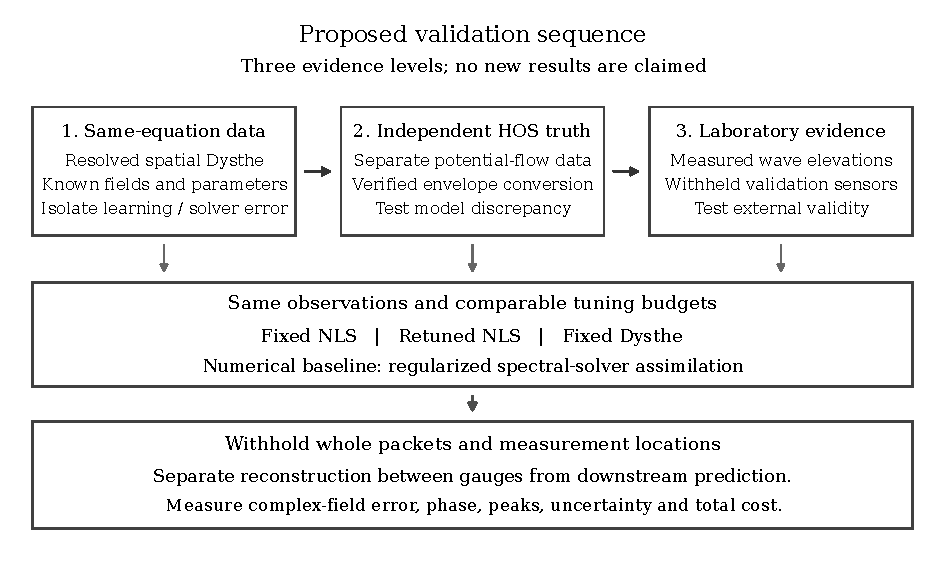
\includegraphics[width=\textwidth]{figures/experiment-design.pdf}
\caption{Proposed study design. Same-equation synthetic tests establish
implementation accuracy; independently generated HOS and laboratory data
address different model-validity questions. These levels must keep their
original physical provenance. The diagram contains no experimental results.}
\label{fig:design}
\end{figure}

\begin{enumerate}
\item \textbf{Numerical accuracy for the declared equation.}
Use plane waves and the mathematical NLS control for elementary checks,
then converged Dysthe packet trajectories. Independently refine
propagation step, profile resolution, nonlinear quadrature, and domain
length. Agreement with one's own unresolved training data is insufficient.
\item \textbf{Approximation of more complete water-wave physics.}
Use HOS truth with its original model label and a documented envelope
extraction map. The public dataset \cite{hosdata} is a candidate source,
not automatically a Dysthe benchmark. Select compatible unidirectional,
deep-water, narrowband cases and justify the validity bounds.
\item \textbf{Measurement performance.}
Use laboratory observations with calibration and noise information.
Assess only quantities independently observed or otherwise supported.
Reconstructing an unmeasured latent potential is not its experimental
validation. Do not make operational sea-state claims from tank data alone.
\end{enumerate}

\subsection{Minimal pilot before a large campaign}
The following is a proposed workload, not an existing result or a universal
sample-size requirement. Begin with three regimes spanning low to moderate
steepness/bandwidth within justified limits, two gauge separations, two
noise levels, and five independently drawn packets per cell:
$3\times2\times2\times5=60$ inverse cases. The noise-free level checks
implementation; the other should reflect an explicit sensor-noise model.
Choose physical parameter values only after reference-resolution and
envelope-validity checks. The $60$ cases are for feasibility, not enough
by themselves to settle all regime interactions.

Run the three equation arms and two inference engines of Question 1.
Start with a few optimizer seeds on the pilot, then choose replication
from observed variability. For the final comparison, use paired initial
fields and noise realizations, report median and upper-tail errors, and
bootstrap whole trajectories rather than individual grid points.
Record optimization failures; do not discard them from the success rate.
A larger study can use a space-filling design followed by targeted
sampling near changes in the relative model performance.

\subsection{A practical PINN starting recipe}
The following is a proposed baseline assembled from inspected methods;
its Dysthe performance remains to be established.
\begin{enumerate}
\item \textbf{Scale the problem.}
Use the recorded physical normalization, nondimensional coordinates,
and training-only feature scaling. Start with double precision for
reference and residual qualification, then measure whether reduced
precision preserves the required accuracy.
\item \textbf{Represent periodicity correctly.}
For an exact periodic inlet $u_0$, use commensurate features such as
$\cos(2\pi\tau/L),\sin(2\pi\tau/L)$ and an ansatz
\[
 u_\theta(\xi,\tau)=u_0(\tau)
       +\frac{\xi}{\Xi}N_\theta\!\left(
          \frac{\xi}{\Xi},\cos(2\pi\tau/L),\sin(2\pi\tau/L)\right),
 \quad 0\leq\xi\leq\Xi .
\]
This enforces the initial field and periodic profile by construction.
If $u_0$ is uncertain, infer a latent inlet and penalize its disagreement
with measurements according to the noise model instead of hard-coding
noisy observations. Random Fourier frequencies are not automatically
periodic with period $L$.
\item \textbf{Evaluate the nonlocal term on complete slices.}
Evaluate the field on a uniform periodic profile grid at sampled
$\xi$ values, apply a differentiable FFT multiplier, and evaluate
products using justified anti-aliasing/projection choices. Validate the
result independently on a finer grid. Record that the residual contains
a numerical spectral operator.
\item \textbf{Use a credible optimizer comparison.}
Compare an Adam-to-L-BFGS recipe with self-scaled Broyden and, if resources
permit, SOAP. Resampling changes the optimization objective and may
interact with quasi-Newton history; specify when points are frozen or
history is reset. Count line searches and derivative evaluations.
\item \textbf{Add complexity one ingredient at a time.}
After the basic model works, test $\xi$ slabs/causal weights, complex
layers, adaptive sampling, and appropriate invariant penalties. Tune
each on validation cases. A large combination without ablations does
not explain why a method works.
\end{enumerate}

\subsection{Metrics that match the scientific claim}
Let $u$ denote a resolved reference and $\widehat u$ a prediction on a
fixed evaluation domain $\Omega$, with physical quadrature weights.
Report at least
\begin{align}
 E_{\rm field}&=\frac{\norm{\widehat u-u}_{L^2(\Omega)}}
                         {\norm{u}_{L^2(\Omega)}},&
 E_{\rm amp}&=\frac{\norm{|\widehat u|-|u|}_{L^2(\Omega)}}
                         {\norm{u}_{L^2(\Omega)}}. \label{eq:metrics}
\end{align}
For meaningful phase evaluation define
$A_\eta=\{(\xi,\tau):|u|\geq\eta,\ |\widehat u|\geq\eta\}$
using a documented amplitude threshold and use, for example,
\[
 E_\phi^2=
 \frac{\int_{A_\eta}|u|^2
     \Arg(\widehat u\,\overline u)^2\dd\xi\dd\tau}
      {\int_{A_\eta}|u|^2\dd\xi\dd\tau}.
\]
If the denominator vanishes, report the metric as undefined. Also report
the fraction of the domain retained by the threshold. Phase- or
translation-aligned errors can diagnose mistakes, but must be accompanied
by unaligned errors and the fitted shifts.

Additional measurements should include:
\begin{itemize}
\item envelope peak height, focusing distance, retarded-time location,
and event detection precision/recall at preregistered thresholds;
\item profile spectra and spectral-edge content; correct invariant
defects, interpreted alongside reference discretization error;
\item withheld surface-elevation error after a fixed observation map;
SSP may aid comparison with water-wave papers but is not interchangeable
with complex-field relative $L^2$ error;
\item coefficient recovery and calibrated interval coverage when
parameters are actually identifiable;
\item training, tuning, data-generation, adaptation and inference time,
peak memory, and total residual/operator evaluations.
\end{itemize}
Never label a small invariant defect, a low training loss, or a visually
plausible envelope an accuracy certificate.

\subsection{Fair comparisons and explicit decision gates}
Separate a best-accuracy experiment from a fixed-budget experiment.
Allow comparable hyperparameter-selection resources, keep the final
test set untouched, and disclose hardware and numerical precision.
Charge adaptive candidate scoring and sampler maintenance
\cite{operatorbudget}; iteration counts alone can hide significant costs.

Before the final campaign, choose a minimum practically useful improvement
and tolerable cost ratio. For example, a \emph{proposed} pilot continuation
rule could require a $20\%$ reduction in median held-out phase or
field error, a paired confidence interval excluding no improvement, and
no material degradation in upper-tail event error. This number is a
project decision to be justified, not a literature standard. If the
reference uncertainty is comparable to the claimed improvement, tighten
the reference first. If no practically useful gain appears, simplify
the method or redirect to the documented identifiability limitation.

\clearpage
\section{Roadmap, current assets, and delivery limits}
\subsection{A staged route to a submission}
The schedule below is an indicative planning estimate, conditional on
compute, data access, and successful validation.
\begin{longtable}{@{}P{0.15\textwidth}P{0.43\textwidth}P{0.34\textwidth}@{}}
\toprule
Stage & Deliverable & Gate before proceeding \\
\midrule
\endfirsthead
\toprule
Stage & Deliverable & Gate before proceeding \\
\midrule
\endhead
Weeks 1--2 & Reproduce one direct NLS baseline; verify the exact
Dysthe residual and observation conversion. & Correct signs, mean flow,
boundary conditions, and independent refinement evidence. \\
Weeks 3--4 & Numerical assimilation and modern PINN pilot;
local sensitivity/identifiability analysis. & Equal observations and
credible simpler-model controls; meaningful effect size. \\
Weeks 5--7 & Expand regimes, seeds, and held-out packets;
one targeted ablation from Question 3. & Stable gains or a robust,
explainable failure boundary. \\
Weeks 8--10 & External HOS or laboratory validation; uncertainty
and cost evaluation; manuscript and reproducibility package. &
Claims match the actual evidence level and survive negative controls. \\
Later & Operator amortization or rigorous certification. &
Strong first-stage baselines; separate novelty and feasibility review. \\
\bottomrule
\end{longtable}

Do not begin all five questions simultaneously. Question 1 with a focused
part of Question 2 supplies a coherent first manuscript. Question 3 can
provide a method explanation if the pilot identifies a genuine training
bottleneck. Question 4 becomes sensible only when repeated-query demand
and dataset costs are known; Question 5 is a separate mathematical track.

\subsection{What is available locally now}
Read-only inspection of the current family confirmed the model contract
and an implemented \texttt{SpatialDysthe} reference solver in
\path{dysthe-core/src/dysthe_core/reference/spatial.py}.
The equation specification is
\path{dysthe-core/docs/model.md}; qualification guidance is
\path{dysthe-core/docs/stage-one-reference.md}.
The FNO and hybrid method READMEs in \texttt{dysthe-learning} still describe
planned methods. This is a current file inspection, not a fresh numerical
qualification or training result. Historical artifacts must retain their
actual equation labels.

The current solver is therefore a starting asset to qualify, rather than
a reason to build an unrelated simulator. The paper should use
\texttt{dysthe-experiments} for frozen campaigns and splits,
\texttt{dysthe-learning} for compared methods, and
\texttt{dysthe-paper} for numerical evidence once experiments exist.
This review does not modify those implementations or assert that the
proposed experiments have been completed.

\subsection{Verification and limitations of this review}
This report provides live primary-source literature checking, access and
status distinctions, explicit future-work provenance, an independent
check of the elementary NLS example and estimate, and original vector
figures. Several very recent Elsevier/Springer papers were accessible
only through abstracts and previews; their full comparative claims,
code, and statistical evidence could not be audited. The stronger
full-text sources and those preview-only leads are identified separately.

No literature experiment, public training code, HOS dataset, or local
solver qualification campaign was rerun. No definitive claim of novelty,
universal best method, ocean-operational readiness, or established
Dysthe--PINN advantage is made. The main deliverable is a concrete,
testable research program grounded in the verified sources below.

\begin{thebibliography}{99}
\addcontentsline{toc}{section}{References}
\setlength{\itemsep}{0.6em}

\bibitem{ehlers2024}
Svenja Ehlers, Niklas A. Wagner, Annamaria Scherzl, Marco Klein, Norbert Hoffmann, and Merten Stender.
\emph{Data Assimilation and Parameter Identification for Water Waves Using the Nonlinear Schr\"{o}dinger Equation and Physics-Informed Neural Networks}.
Fluids 9(10), 231 (2024).
\href{https://doi.org/10.3390/fluids9100231}{\nolinkurl{10.3390/fluids9100231}}.

\bibitem{ehlers2025}
Svenja Ehlers, Norbert Hoffmann, Tianning Tang, Adrian H. Callaghan, Rui Cao, Enrique M. Padilla, Yuxin Fang, and Merten Stender.
\emph{Physics-informed neural networks for phase-resolved data assimilation and prediction of nonlinear ocean waves}.
Physical Review Fluids 10, 094901 (2025).
\href{https://doi.org/10.1103/ytyy-pvys}{\nolinkurl{10.1103/ytyy-pvys}}.

\bibitem{wavepino}
Svenja Ehlers, Merten Stender, and Norbert Hoffmann.
\emph{Bridging ocean wave physics and deep learning: Physics-informed neural operators for nonlinear wavefield reconstruction in real-time}.
Physics of Fluids 37(10), 107119 (2025).
\href{https://doi.org/10.1063/5.0294655}{\nolinkurl{10.1063/5.0294655}}.

\bibitem{urban}
Jorge F. Urb\'{a}n, Petros Stefanou, and Jos\'{e} A. Pons.
\emph{Unveiling the optimization process of physics informed neural networks: How accurate and competitive can PINNs be?}.
Journal of Computational Physics 523, 113656 (2025).
\href{https://doi.org/10.1016/j.jcp.2024.113656}{\nolinkurl{10.1016/j.jcp.2024.113656}}.

\bibitem{cvpinn}
Lei Zhang, Mengge Du, Xiaodong Bai, Yuntian Chen, and Dongxiao Zhang.
\emph{Complex-valued physics-informed machine learning for efficient solving of quintic nonlinear Schr\"{o}dinger equations}.
Physical Review Research 7, 013164 (2025).
\href{https://doi.org/10.1103/PhysRevResearch.7.013164}{\nolinkurl{10.1103/PhysRevResearch.7.013164}}.

\bibitem{hardic}
Baoli Hao, Chun Liu, Ulisses Braga-Neto, Lifan Wang, and Ming Zhong.
\emph{Stability in training PINNs for stiff PDEs: Why initial conditions matter}.
Foundations of Data Science, early access (2026).
\href{https://doi.org/10.3934/fods.2026016}{\nolinkurl{10.3934/fods.2026016}}.

\bibitem{alejo}
Miguel \'{A}. Alejo, Lucrezia Cossetti, Luca Fanelli, Claudio Mu\~{n}oz, and Nicol\'{a}s Valenzuela.
\emph{Error bounds for Physics Informed Neural Networks in Nonlinear Schr\"{o}dinger equations placed on unbounded domains}.
arXiv:2409.17938v3, preprint; first submitted 2024 (2025).
\href{https://doi.org/10.48550/arXiv.2409.17938}{\nolinkurl{10.48550/arXiv.2409.17938}}.

\bibitem{eiras}
Francisco Eiras, Adel Bibi, Rudy R. Bunel, Krishnamurthy Dj Dvijotham, Philip Torr, and M. Pawan Kumar.
\emph{Efficient Error Certification for Physics-Informed Neural Networks}.
Proceedings of the 41st International Conference on Machine Learning, PMLR 235, 12318--12347 (2024).
\href{https://proceedings.mlr.press/v235/eiras24a.html}{Primary record}.

\bibitem{raissi}
Maziar Raissi, Paris Perdikaris, and George Em Karniadakis.
\emph{Physics-informed neural networks: A deep learning framework for solving forward and inverse problems involving nonlinear partial differential equations}.
Journal of Computational Physics 378, 686--707 (2019).
\href{https://doi.org/10.1016/j.jcp.2018.10.045}{\nolinkurl{10.1016/j.jcp.2018.10.045}}.

\bibitem{pino}
Zongyi Li, Hongkai Zheng, Nikola Kovachki, David Jin, Haoxuan Chen, Burigede Liu, Kamyar Azizzadenesheli, and Anima Anandkumar.
\emph{Physics-Informed Neural Operator for Learning Partial Differential Equations}.
ACM/IMS Journal of Data Science (2024).
\href{https://doi.org/10.1145/3648506}{\nolinkurl{10.1145/3648506}}.

\bibitem{fedele}
Francesco Fedele, and Denys Dutykh.
\emph{Hamiltonian description and traveling waves of the spatial Dysthe equations}.
arXiv:1110.3605v3, research report; first submitted 17 October 2011 (2012).
\href{https://doi.org/10.48550/arXiv.1110.3605}{\nolinkurl{10.48550/arXiv.1110.3605}}.

\bibitem{causal}
Sifan Wang, Shyam Sankaran, and Paris Perdikaris.
\emph{Respecting causality for training physics-informed neural networks}.
Computer Methods in Applied Mechanics and Engineering 421, 116813 (2024).
\href{https://doi.org/10.1016/j.cma.2024.116813}{\nolinkurl{10.1016/j.cma.2024.116813}}.

\bibitem{gravis}
Long Chen, Fan Liu, Yongming Zhang, and Weiqi Chen.
\emph{Physics-informed neural networks for nonlinear Schr\"{o}dinger localized wave problems with gradient-residual adaptive collocation sampling}.
Nonlinear Dynamics 114, 820 (2026).
\href{https://doi.org/10.1007/s11071-026-12723-1}{\nolinkurl{10.1007/s11071-026-12723-1}}.

\bibitem{soap}
Sifan Wang, Ananyae Kumar Bhartari, Bowen Li, and Paris Perdikaris.
\emph{Gradient Alignment in Physics-informed Neural Networks: A Second-Order Optimization Perspective}.
Advances in Neural Information Processing Systems 38, Main Conference (2025).
\href{https://doi.org/10.52202/085713-5615}{\nolinkurl{10.52202/085713-5615}}.

\bibitem{hosdata}
Svenja Ehlers.
\emph{Data to train a physics-informed neural operator for ocean wave reconstruction}.
Zenodo, version 1, dataset (2026).
\href{https://doi.org/10.5281/zenodo.19473989}{\nolinkurl{10.5281/zenodo.19473989}}.

\bibitem{tdd}
Jiaxin Chen, Biao Li, and Manwai Yuen.
\emph{Data-driven SFB solutions and parameters discovery for nonlinear Schr\"{o}dinger equation via time domain decomposition physics-informed neural networks}.
Computers \& Mathematics with Applications 199, 45-63 (issue date) (2025).
\href{https://doi.org/10.1016/j.camwa.2025.09.007}{\nolinkurl{10.1016/j.camwa.2025.09.007}}.

\bibitem{interaction}
Jiaxin Chen, Biao Li, and Manwai Yuen.
\emph{Nonlinear interaction multi-domain physics-informed neural networks for the hybrid rogue wave and breather solutions of the nonlinear Schr\"{o}dinger equation}.
Communications in Nonlinear Science and Numerical Simulation 151, 109049 (2025).
\href{https://doi.org/10.1016/j.cnsns.2025.109049}{\nolinkurl{10.1016/j.cnsns.2025.109049}}.

\bibitem{transfer}
Yikai Chen, Hongli Xiao, Xiao Teng, Wenjun Liu, and Long Lan.
\emph{Enhancing accuracy of physically informed neural networks for nonlinear Schr\"{o}dinger equations through multi-view transfer learning}.
Information Fusion 102, 102041 (2024).
\href{https://doi.org/10.1016/j.inffus.2023.102041}{\nolinkurl{10.1016/j.inffus.2023.102041}}.

\bibitem{noether}
Yanrui Zhang, and Fujun Liu.
\emph{Noether-constrained physics-informed neural networks for the nonlinear Schr\"{o}dinger equation}.
Physics Letters A 589, 131802 (issue date) (2026).
\href{https://doi.org/10.1016/j.physleta.2026.131802}{\nolinkurl{10.1016/j.physleta.2026.131802}}.

\bibitem{cpa}
Shubham Kumar, Himanshu Kumar Dwivedi, and Rajeev.
\emph{Structure-preserving conservative phase-amplitude PINNs for semiclassical Schr\"{o}dinger-type equations}.
Journal of Computational and Applied Mathematics 485, 117607 (issue date) (2026).
\href{https://doi.org/10.1016/j.cam.2026.117607}{\nolinkurl{10.1016/j.cam.2026.117607}}.

\bibitem{extreme2026}
Angeline Hu, Ava K. Tse, Kaitlyn S. Yasumura, Luciana Sarabia, Malcolm Yeung, Kavin K. Prasanna, Kai Wong, William Hammond, Ioannis G. Keverkidis, Shengkai Li, and Trung V. Phan.
\emph{Geometry-Agnostic Data-Driven Discovery of Extreme Scenarios}.
arXiv:2610.28487v1, preprint (2026).
\href{https://doi.org/10.48550/arXiv.2610.28487}{\nolinkurl{10.48550/arXiv.2610.28487}}.

\bibitem{pirate}
Sifan Wang, Bowen Li, Yuhan Chen, and Paris Perdikaris.
\emph{PirateNets: Physics-informed Deep Learning with Residual Adaptive Networks}.
Journal of Machine Learning Research 25(402), 1--51 (2024).
\href{https://jmlr.org/papers/v25/24-0313.html}{Primary record}.

\bibitem{optimizer}
Elham Kiyani, Khemraj Shukla, Jorge F. Urb\'{a}n, J\'{e}r\^{o}me Darbon, and George Em Karniadakis.
\emph{Optimizing the optimizer for physics-informed neural networks and Kolmogorov-Arnold networks}.
Computer Methods in Applied Mechanics and Engineering 446, 118308 (2025).
\href{https://doi.org/10.1016/j.cma.2025.118308}{\nolinkurl{10.1016/j.cma.2025.118308}}.

\bibitem{pinnacle}
Zhongkai Hao, Jiachen Yao, Chang Su, Hang Su, Ziao Wang, Fanzhi Lu, Zeyu Xia, Yichi Zhang, Songming Liu, Lu Lu, and Jun Zhu.
\emph{PINNacle: A Comprehensive Benchmark of Physics-Informed Neural Networks for Solving PDEs}.
NeurIPS 2024 Datasets and Benchmarks (2024).
\href{https://papers.nips.cc/paper/2024/file/8c63299fb2820ef41cb05e2ff11836f5-Paper-Datasets_and_Benchmarks_Track.pdf}{Primary record}.

\bibitem{spectral}
Tianchi Yu, Yiming Qi, Ivan Oseledets, and Shiyi Chen.
\emph{Spectral informed neural networks}.
Journal of Computational and Applied Mathematics 477, 117178 (2026).
\href{https://doi.org/10.1016/j.cam.2025.117178}{\nolinkurl{10.1016/j.cam.2025.117178}}.

\bibitem{goal}
Medard Govoeyi, and Thomas Richter.
\emph{Goal oriented error estimation for adaptive sampling of PINNS}.
arXiv preprint, math.NA, 2604.01835v1 (2026).
\href{https://doi.org/10.48550/arXiv.2604.01835}{\nolinkurl{10.48550/arXiv.2604.01835}}.

\bibitem{operatorbudget}
Yifei Long, and Kuan Fan.
\emph{Operator-Budget Evaluation of Residual-Adaptive Sampling in Physics-Informed Neural Networks}.
Applied Sciences 16(19), 9508 (2026).
\href{https://doi.org/10.3390/app16199508}{\nolinkurl{10.3390/app16199508}}.

\bibitem{grossmann}
Tamara G. Grossmann, Urszula Julia Komorowska, Jonas Latz, and Carola-Bibiane Sch\"{o}nlieb.
\emph{Can physics-informed neural networks beat the finite element method?}.
IMA Journal of Applied Mathematics 89(1), 143--174 (2024).
\href{https://doi.org/10.1093/imamat/hxae011}{\nolinkurl{10.1093/imamat/hxae011}}.

\end{thebibliography}

\end{document}
